\documentclass{article}
\usepackage[utf8]{inputenc}
\usepackage{graphicx}
\usepackage{amsmath}
\usepackage{amssymb}
\usepackage{amsthm}
\usepackage{bm}

\title{Computational Physics (physics760)\\Exercise 5}
\author{Ajay S. Sakthivasan, Dongjin Suh}
\date{December 2, 2022}

\begin{document}

\maketitle

\begin{enumerate}
\item \textbf{Artifical Hamiltonian and its corresponding equations of motion}\\
\begin{flalign*}
&\text{The action:} &\\ 
&S[\Phi] = \Phi^{2} &\\
\\
&\text{The artifical Hamiltonian:} &\\
&\mathcal{H} = \quad \frac{p^2}{2} + S[\Phi] \quad = \quad \frac{p^2}{2} + \Phi^{2} &\\
\\
&\text{Hamiltonian's equations of motion: }&\\
&(1)\quad\dot{\phi} = \frac{\partial}{\partial p} \mathcal{H} = p&\\
&(2)\quad\dot{p} = -\frac{\partial}{\partial \phi} \mathcal{H} = -2\Phi &\\
\end{flalign*}

\item \textbf{Leapfrog Integrator}\\
Modifying the leapfrog integrator to accommodate the new system in-hand, we obtain plot \ref{fig:leapfrog} for relative error vs. molecular dynamics steps. Figure \ref{fig:hmc} shows the observable plotted against the HMC trajectory. We then compare the autocorrelation function with the function $\exp{(t/\tau_{int})}$ for $t\geq 0$. This is given in figure \ref{fig:autocorr-exp}. We can also see from figure \ref{fig:autocorr-bin} that the autocorrelation decreases as the bin width is increased.\\

\begin{figure}[h!]
    \centering
    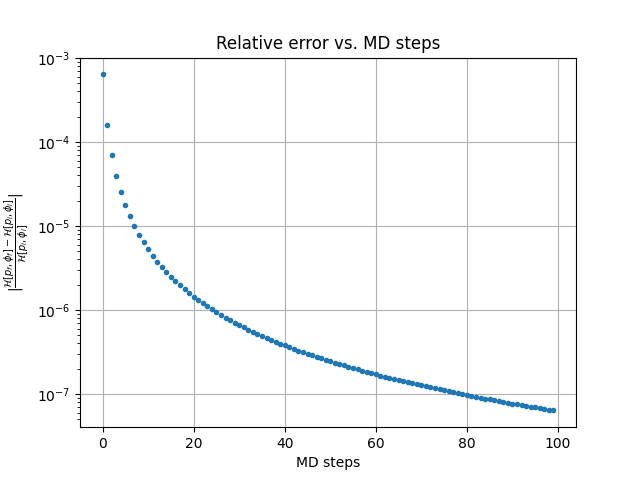
\includegraphics[width=.8\linewidth]{leapfrog.png}
    \caption{Relative Error vs. MD steps obtained from Leapfrog integrator}
    \label{fig:leapfrog}
\end{figure}

\begin{figure}[h!]
    \centering
    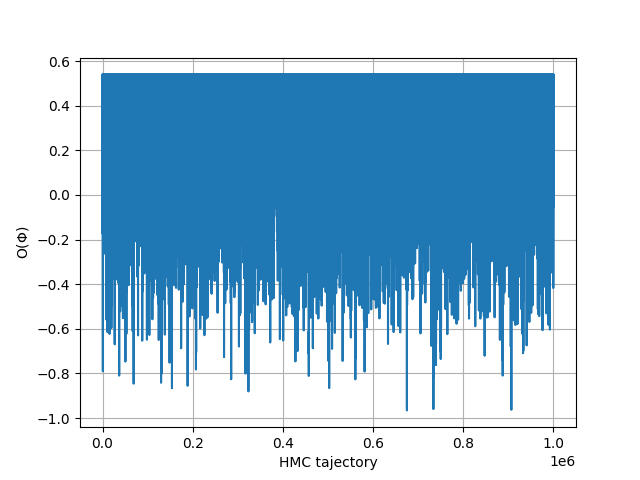
\includegraphics[width=.8\linewidth]{observable_markov_chain_1mio.png}
    \caption{Observable vs. HMC trajectory}
    \label{fig:hmc}
\end{figure}

\begin{figure}[h!]
    \centering
    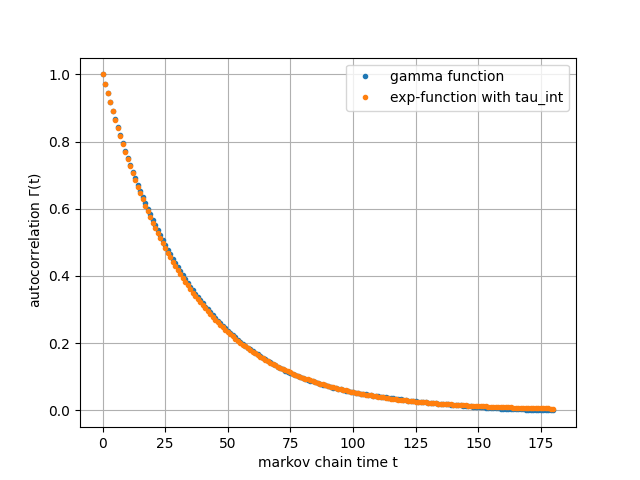
\includegraphics[width=.8\linewidth]{autocorr_func_vs_tau_int.png}
    \caption{Autocorrelation vs. Markov Chain Time}
    \label{fig:autocorr-exp}
\end{figure}

\begin{figure}[h!]
    \centering
    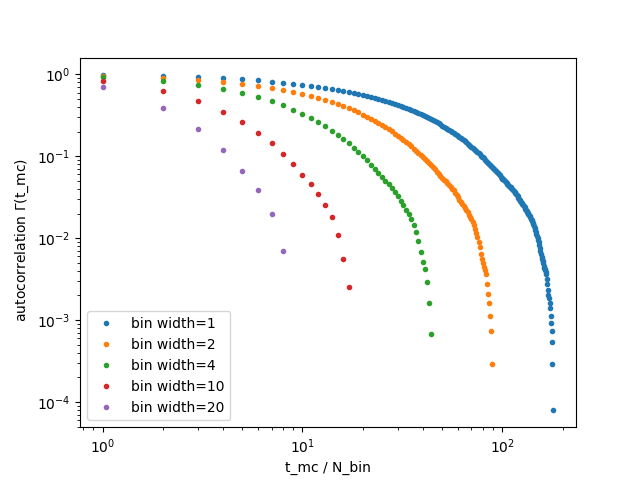
\includegraphics[width=.8\linewidth]{autocorr_different_binwidth.png}
    \caption{Autocorrelation vs. Markov Chain Time for different Bin Widths}
    \label{fig:autocorr-bin}
\end{figure}

\clearpage
\item \textbf{Bootstrap Routine}\\


\end{enumerate}

\end{document}